\documentclass[xcolor={usenames,dvipsnames,svgnames}, compress]{beamer}

\usepackage{booktabs}
\usepackage{dcolumn}
\usepackage{colortbl}
\usepackage{xcolor}
\usepackage{hyperref}
\usepackage{amsmath}
\usepackage{wrapfig}
\usepackage{pifont}
\usepackage[style=authoryear-comp]{biblatex}

\usepackage[font=scriptsize]{caption}

% 
% custom colors
\definecolor{untractable_red}{RGB}{209, 25, 25}
\definecolor{tractable_green}{RGB}{0, 153, 51}

\usetheme{enziteto}

\setbeamertemplate{headline}{}

% 
% custom colors
\definecolor{untractable_red}{RGB}{209, 25, 25}
\definecolor{tractable_green}{RGB}{0, 153, 51}

\newcommand{\cmark}{\ding{51}}%
\newcommand{\xmark}{\ding{55}}

\addbibresource{../referomnia/referomnia.bib}

\begin{document}

\newlength{\custombulletheight}
\setlength{\custombulletheight}{\dimexpr0.5\ht1-0.5\ht2}

\title{Fast and Accurate Denstiy Estimation with Extremely Randomized
  Cutset Networks}
\author{Nicola  {Di Mauro}, Antonio  Vergari, Teresa M.A. Basile and Floriana Esposito}
\date{}
\institute{Lacam$@$DIB$@$Uniba}
\institute{Università degli Studi di Bari}
\department{Dipartimento di Informatica}
\laboratory{LACAM Laboratory}
\group{Machine Learning}
\institutelogo{
\includegraphics[width=25pt]{figures/unibaba}}
\lablogo{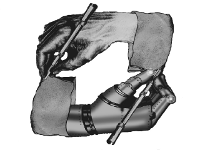
\includegraphics[width=35pt]{figures/lacam}}
\date{19th September - \textbf{ECML-PKDD 2017} - Skopje, Macedonia}


{
  \setbeamertemplate{headline}{}
  \setbeamertemplate{footline}{}
  \begin{frame}
    \titlepage
  \end{frame}
}

\begin{frame}[t]
  \frametitle{Outline}
  
\end{frame}


\begin{frame}[t]
  \frametitle{Density Estimation}
  
\end{frame}

\begin{frame}[t]
  \frametitle{Tractable Probabilistic Models (TPMs)}
  
\end{frame}

\begin{frame}[t]
  \frametitle{Cutset Networks (CNets)}
  
\end{frame}

\begin{frame}[t]
  \frametitle{Learning CNets}
  
\end{frame}

\begin{frame}[t]
  \frametitle{XCNets}
  
\end{frame}

\begin{frame}[t]
  \frametitle{Mixture of Experts}
  
\end{frame}

\begin{frame}[t]
  \frametitle{Regularization}
  
\end{frame}


\begin{frame}[t]
  \frametitle{Single Model Comparison}
  
\end{frame}

\begin{frame}[t]
  \frametitle{Ensemble Model Comparison}
  
\end{frame}

\begin{frame}[t]
  \frametitle{Learning Times}
  
\end{frame}

\begin{frame}[t]
  \frametitle{Conclusions}
  
\end{frame}







% \begin{frame}[t]
%   \frametitle{Tractable Probabilistic Models (TPMs)}
%   \small
%   Plenty of Probabilistic Models learned as \emph{density estimators}\\[6pt]
  
%   Many Machine Learning problems can be reframed as probabilitic
%   inference\\[6pt]
   
%    \dots but \emph{\textbf{inference is hard}}.
%    \begin{center}
%     \begin{minipage}[t]{0.29\linewidth}
%       \begin{center}
%         \includegraphics[width=0.8\linewidth]{figures/tree}\\
%         % \begin{minipage}[t]{0.58\linewidth}
%         %   \scriptsize \flushleft
%         %   \textcolor{tractable_green}{\cmark \textbf{EVI}},
%         %   \textcolor{tractable_green}{\cmark \textbf{SAM}},
%         %   \textcolor{tractable_green}{\cmark \textbf{MAR}},\par
%         %   \textcolor{tractable_green}{\cmark \textbf{CON}},
%         %   \textcolor{tractable_green}{\cmark \textbf{MPE}},
%         %   \textcolor{tractable_green}{\cmark \textbf{Z}}
%         % \end{minipage}
%         \textbf{\emph{\textcolor{tractable_green}{Low treewidth PGMs}}}\\[20pt]
%       \end{center}
%     \end{minipage}\hfill\begin{minipage}[t]{0.32\linewidth}
%       \begin{center}
%         \includegraphics[width=0.7\linewidth]{figures/spn}\\
%         % \begin{minipage}[t]{0.48\linewidth}
%         %   \scriptsize \flushleft
%         %   \textcolor{tractable_green}{\cmark \textbf{EVI}},
%         %   \textcolor{tractable_green}{\cmark \textbf{SAM}},
%         %   \textcolor{tractable_green}{\cmark \textbf{MAR}},\par
%         %   \textcolor{tractable_green}{\cmark \textbf{CON}},
%         %   \textcolor{untractable_red}{\xmark \textbf{MPE}},
%         %   \textcolor{tractable_green}{\cmark \textbf{Z}}
%         % \end{minipage}
%         \textbf{\emph{\textcolor{tractable_green}{Computational Graphs}}}\\[20pt]
%       \end{center}
%     \end{minipage}\hfill\begin{minipage}[t]{0.29\linewidth}
%       \begin{center}
%         \includegraphics[width=0.8\linewidth]{figures/nade}\\
%         % \begin{minipage}[t]{0.57\linewidth}
%         %   \scriptsize \flushleft
%         %   \textcolor{tractable_green}{\cmark \textbf{EVI}},
%         %   \textcolor{tractable_green}{\cmark \textbf{SAM}},
%         %   \textcolor{untractable_red}{\xmark \textbf{MAR}},\par
%         %   \textcolor{untractable_red}{\xmark \textbf{CON}},
%         %   \textcolor{untractable_red}{\xmark \textbf{MPE}},
%         %   \textcolor{untractable_red}{\xmark \textbf{Z}}
%         % \end{minipage}
%         \textbf{\emph{\textcolor{tractable_green}{Autoregressive NNs}}}\\[20pt]
%       \end{center}
%     \end{minipage}
%   \end{center}\vspace{7pt}
%   $\rightarrow$ TPMs allow \textbf{exact} inference to be computed in \textbf{\textcolor{tractable_green}{polynomial time}}!
% \end{frame}


\end{document}

%%% Local Variables:
%%% mode: latex
%%% TeX-engine: xetex
%%% TeX-master: t
%%% End:
